\section{Remarks on the Scalar \texorpdfstring{$u$}{u}}
\label{sec:scalar}

Each remark below is a reading of $u = \rho\,\sech\tau$.
None of them adds a second coordinate.

\subsection{Affine Reciprocal}

From \cref{eq:canonical},
\begin{equation}
  \frac{1}{\eta} = 1 - \rho\,\sech\tau = 1 - u.
  \label{eq:reciprocal_linear}
\end{equation}
At fixed $\tau$, $1/\eta$ is an affine function of $\rho$.
A level set of $1/\eta$ is a line in that coordinate, not a plane.
The curvature of iso-$\eta$ contours in the $(\tau,\rho)$-plane is the image of that line under $\rho \mapsto \rho\,\sech\tau$.
\Cref{fig:mobius} shows both pictures.

\begin{figure}[t]
  \centering
  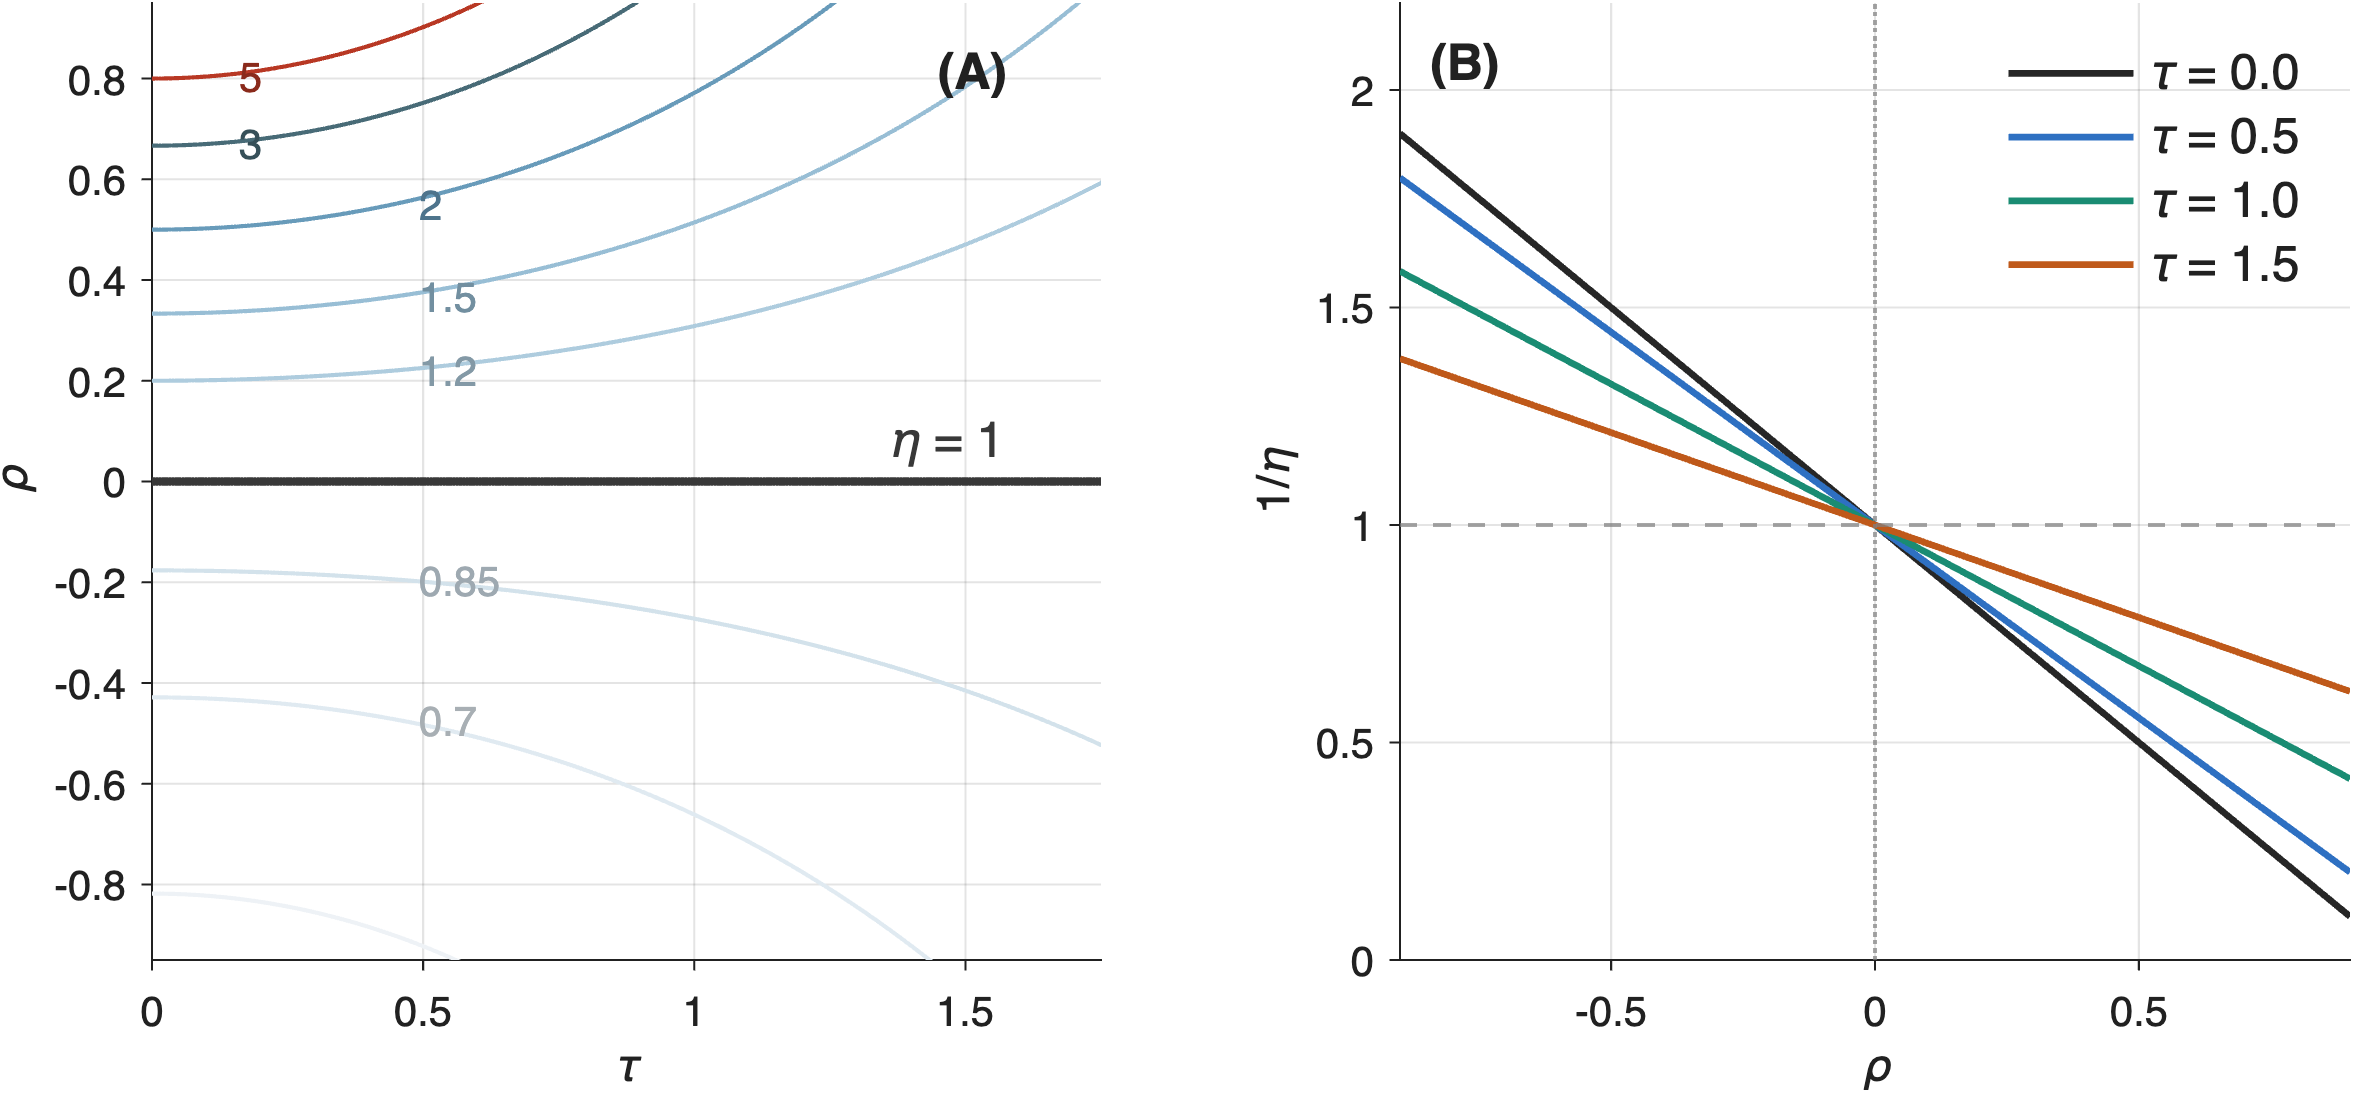
\includegraphics[width=\textwidth]{figures/Figure_2_mobius_linearisation.png}
  \caption{The reciprocal is affine in $\rho$ at fixed $\tau$.
    (A)~Iso-$\eta$ contours $\rho = (1-1/\eta)\cosh\tau$ on the half-strip.
    (B)~$1/\eta = 1-\rho\,\sech\tau$ at four fixed values of $\tau$.}
  \label{fig:mobius}
\end{figure}

\subsection{Poisson Kernel on the Inner Disc}

The classical Poisson kernel $P_{s}(\varphi) = (1-s^{2})/|1-s\,e^{i\varphi}|^{2}$ is positive for $0\le s<1$.
On the fundamental domain $\tau>0$ one has $r = e^{\tau}>1$, so the kernel at radius $r$ is not the disc kernel.
Apply \cref{thm:involution} and set $s = e^{-\tau}\in(0,1)$, with $\rho = \cos\varphi$:
\begin{equation}
  \eta(\tau,\rho)
  = \coth\tau\; P_{e^{-\tau}}(\varphi),
  \qquad \tau>0.
  \label{eq:eta_poisson_ratio}
\end{equation}
Since $\coth\tau>1$ for $\tau>0$, one has $\eta > P_{e^{-\tau}}(\varphi)$ on the open half-strip.
The ratio $\eta/P_{e^{-\tau}}(\varphi)$ tends to $1$ only as $\tau\to\infty$.
As $\tau\to 0^{+}$, $\coth\tau\to\infty$ and the product tends to Fisher's value $1/(1-\rho)$.
The factor $\eta$ is not itself harmonic.
It is a harmonic function multiplied by $\coth\tau$.

\subsection{Geometric Series}

Whenever $|u|<1$,
\begin{equation}
  \eta(\tau,\rho) = \frac{1}{1-u} = \sum_{k=0}^{\infty}(\rho\,\sech\tau)^{k}.
  \label{eq:geometric_series}
\end{equation}
In the open physical domain the bound holds for every admissible $(\tau,\rho)$: $|\rho\,\sech\tau| \le \sech\tau < 1$ when $\tau>0$, and $|\rho|<1$ when $\tau = 0$ except at the pole $\rho\to 1$.
On the branch $\kappa<1$ the same rational function is $(1+r^{2})\sum_{n=0}^{\infty} U_{n}(\rho)\, r^{n}$ with $r = \sqrt{\kappa}$, where $U_{n}$ is the Chebyshev polynomial of the second kind \parencite{rivlin1990}.
Both series are rearrangements of \cref{eq:pef_original}.

\subsection{Latitudes}
\label{sec:sphere_remark}

Set $\cos\sigma = u$ with $\sigma\in(0,\pi)$.
Then $\eta = 1/(1-\cos\sigma)$.
Any value of $u$ in $(-1,1)$ is a cosine, and the longitude is not determined by $(\kappa,\rho)$.
Iso-$\eta$ sets are latitudes because $\eta$ depends on $\sigma$ alone.
The construction does not send $(\kappa,\rho)$ to a point of the sphere, and it does not use a complex structure.
The involution $\tau\mapsto-\tau$ preserves $u$, so it pairs the empirical cell $\kappa>1$ with the cell $\kappa<1$ at the same sign of $\rho$.
It pairs Quadrant~1 with Quadrant~2, and Quadrant~3 with Quadrant~4, in the labelling of \textcite{brownPEFempirical}.
Quadrant~4 is the cell $\kappa>1$, $\rho<0$.
It is not a high-asymmetry cell with $\kappa\approx 1$.

\subsection{Latent Geometric Family}
\label{sec:latent_family}

For $u\in(0,1)$, set $\theta = \log u < 0$ and $A(\theta) = -\log(1-e^{\theta})$.
Then $A(\theta) = \log\eta$, and
\begin{equation}
  p(n;\theta) = (1-e^{\theta})\, e^{n\theta}, \qquad n = 0,1,2,\ldots,
  \label{eq:geo_family}
\end{equation}
is a geometric family with natural parameter $\theta$ and mean $A'(\theta) = \eta-1$.
The variance is $A''(\theta) = \eta(\eta-1)$.
The count $N$ is a latent variable attached to $\eta$.
It is not a function of the paired sample $(X_{\mathrm{A}},X_{\mathrm{B}})$.
For $\rho\le 0$ one has $u\le 0$, so $\theta = \log u$ is undefined and \cref{eq:geo_family} does not exist.

The cumulant identities are algebraic consequences of $\eta = 1/(1-u)$ on $u\in(0,1)$.
They carry no information about a match outcome.
In particular they are unrelated to $I(X;Y)$ in \textcite{brownPEFempirical}, which depends on the mean separation.
The Gaussian mutual information of the two margins is $-\tfrac{1}{2}\log(1-\rho^{2})$.
That quantity does not depend on $\kappa$.
At $\kappa = 1$ one has $\log\eta = -\log(1-\rho)$, which is a different function of $\rho$.
